% This file was created by tikzplotlib v0.9.8.
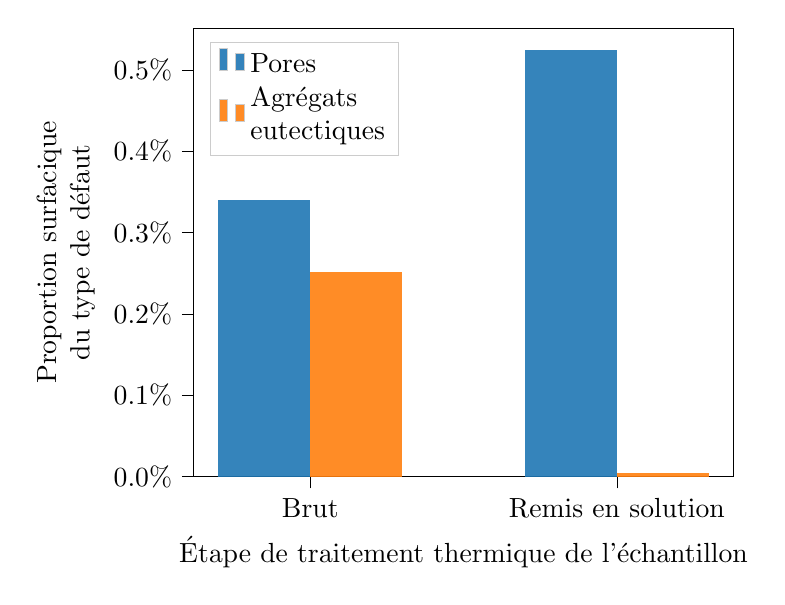
\begin{tikzpicture}

\definecolor{color0}{rgb}{0.12156862745098,0.466666666666667,0.705882352941177}
\definecolor{color1}{rgb}{1,0.498039215686275,0.0549019607843137}

\begin{axis}[
legend cell align={left},
legend style={
  fill opacity=0.8,
  draw opacity=1,
  text opacity=1,
  at={(0.03,0.97)},
  anchor=north west,
  draw=white!80!black
},
tick align=outside,
tick pos=left,
% title={Évolution des défauts dans les échantillons\\selon les traitements thermiques appliqués},
% title style = {align=center},
x grid style={white!69.0196078431373!black},
xlabel={Étape de traitement thermique de l'échantillon},
xmin=-0.23, xmax=1.53,
xtick style={color=black},
xtick={0.15,1.15},
xticklabels={Brut,Remis en solution},
y grid style={white!69.0196078431373!black},
ylabel={Proportion surfacique\\du type de défaut},
% ylabel style={text width=4cm},
ylabel style={align=center},
ymin=0, ymax=0.55125,
ytick style={color=black},
ytick={0,0.1,0.2,0.3,0.4,0.5,0.6},
yticklabels={0.0\%,0.1\%,0.2\%,0.3\%,0.4\%,0.5\%,0.6\%}
]
\draw[draw=none,fill=color0,fill opacity=0.9] (axis cs:-0.15,0) rectangle (axis cs:0.15,0.34);
\addlegendimage{ybar,ybar legend,draw=none,fill=color0,fill opacity=0.9};
\addlegendentry{Pores}

\draw[draw=none,fill=color0,fill opacity=0.9] (axis cs:0.85,0) rectangle (axis cs:1.15,0.525);
\draw[draw=none,fill=color1,fill opacity=0.9] (axis cs:0.15,0) rectangle (axis cs:0.45,0.252);
\addlegendimage{ybar,ybar legend,draw=none,fill=color1,fill opacity=0.9};
\addlegendentry[align=left]{Agrégats\\eutectiques}

\draw[draw=none,fill=color1,fill opacity=0.9] (axis cs:1.15,0) rectangle (axis cs:1.45,0.0041);
\end{axis}

\end{tikzpicture}
